\documentclass[12pt]{article}
\usepackage[margin=1in]{geometry}
\usepackage{graphicx}
\usepackage[T1]{fontenc}
\usepackage[scaled]{beramono}
\usepackage{listings}
\usepackage{amsmath}
\usepackage{amssymb}
\begin{document}

{\centering\noindent\large Iceburg Trajectory Optimization Problem\\
\normalsize Simon Broadhead\\
\today\\}

\vspace{2em}

One major problem in solving a trajectory optimization problem with obstacles is that the feasible region is
non-convex. We can attempt to solve this by breaking the initial problem into several subproblems, each one with a
convex feasible region. The problem then is to determine how the subproblems should be formulated.

In the iceburg problem, we wish to guide an iceburg from a starting position to an ending position while avoiding a
number of polygonal obstacles (see Figure~\ref{fig:base}).
The iceburg is equipped with a boiler which can melt the ice to produce steam propulsion,
resulting in the mass of the iceburg changing over time. We may also introduce other factors, such as water currents or
obstacle movement. For now we will focus on a simplified version of the problem where the mass does not change over time
and the iceburg is an infinitely small point. We will assume that the iceburg is equipped with thrusters so that the 
acceleration can be directly controlled at any given time.
We wish to minimize the total energy expended by the iceburg subject to the constraints that the iceburg's position
at every time is not within any of the polygons, and that the iceburg's thrust is less than some maximum.

Because this is a non-linear problem, the general linear method of hugging the boundaries and jumping directly
from point to point may not be optimal, because, for example, a fast-moving water current may make a more complex path
require less energy than the direct route (in fact a very fortuitous current may take us from the start to the destination
without expending any energy).
However, we can use the points and lines that make up the polygons to decompose the
feasible region into convex subregions in which optimal paths can be computed. The combination of these optimal paths
should hopefully approximate an actual near-optimal solution.

At each step, a convex region containing the current position of the iceburg must be chosen. One way to do this is
to choose one of the polygon points that has an unobstructed straight line to the iceburg, and carve out the largest
convex region that contains both the current point and the target point (see Figure~\ref{fig:step1}).
The optimal path from the current point to the target point can then be computed using convex optimization methods.

Another strategy would be to start by finding a suitably large convex region containing the current point and then
choosing the target point to be the corner of the region closest to the destination (see Figure~\ref{fig:step2}).

The problem of choosing boundary constraints from which to construct the feasible region will require investigation.
Since the number and complexity of the polygons will be limited, a fairly simple enumeration of all of the candidate
boundary constraints at each step should be possible. Alternatively, new constraints
not associated with any of the polygons could be added (see Figure~\ref{fig:step3}).


\begin{figure}[h]
\centering
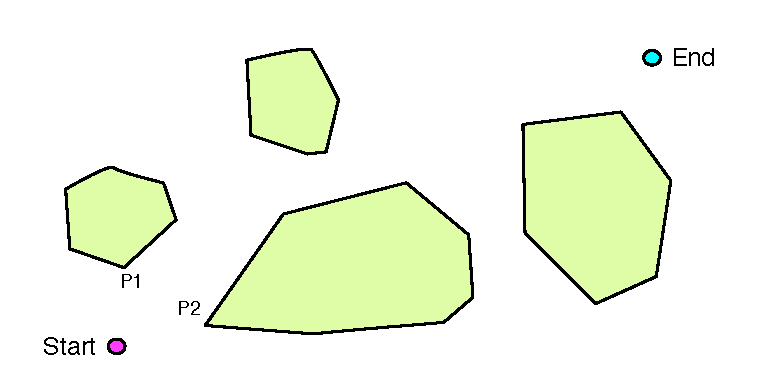
\includegraphics[width=4in]{base}
\caption{The initial layout of the problem.}
\label{fig:base}
\end{figure}

\begin{figure}[h]
\centering
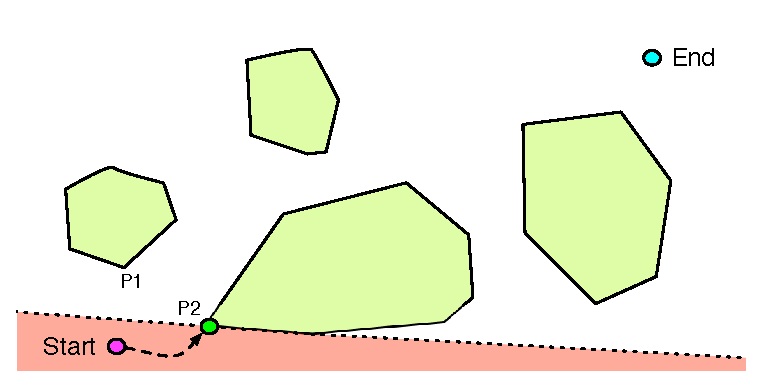
\includegraphics[width=4in]{step1}
\caption{The initial step is taken by choosing a point that is both sufficiently close and which moves the iceburg
in the same general direction as the destination. A convex feasible region (in red) that contains both that point
and the current position of the iceburg is then chosen. The resulting optimization problem then ensures that the
iceburg ends up at the chosen point.}
\label{fig:step1}
\end{figure}


\begin{figure}[h]
\centering
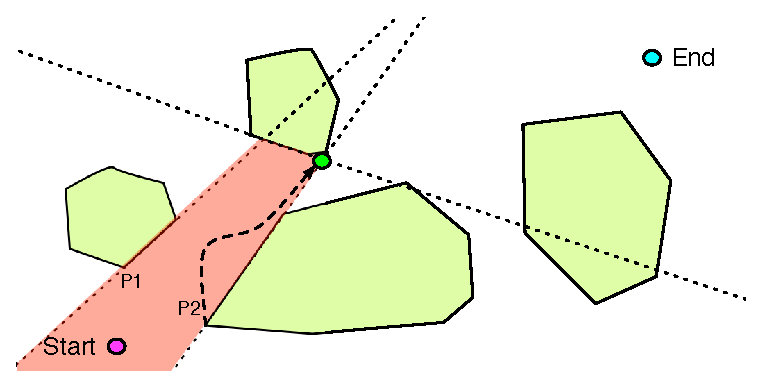
\includegraphics[width=4in]{step2}
\caption{The next step is taken by first constructing a convex feasible region containing the iceburg and then
choosing the target point to be the closest corner to the destination. Note that we could have started with this
step and still ended up in the same place, so this might be a better general strategy.}
\label{fig:step2}
\end{figure}

\begin{figure}[h]
\centering
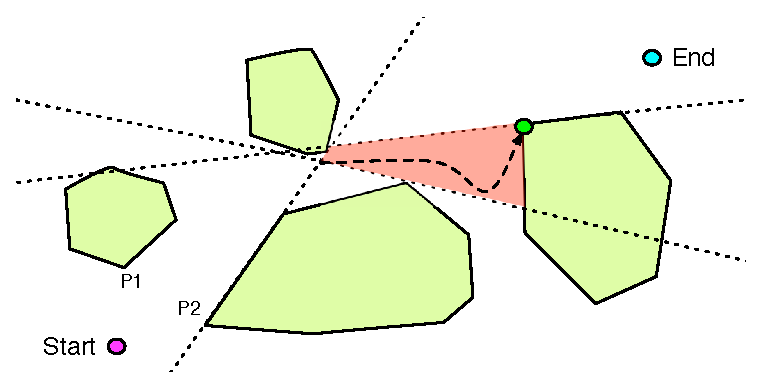
\includegraphics[width=4in]{step3}
\caption{This convex region is constructed by making a new constraint, rather than using only the constraints that make
up the polygons.}
\label{fig:step3}
\end{figure}


\begin{figure}[h]
\centering
\includegraphics[width=4in]{step4}
\caption{The final step.}
\label{fig:step4}
\end{figure}




\end{document}
